\section{Auswertung}
\label{sec:Auswertung}

\begin{figure}
	\centering
	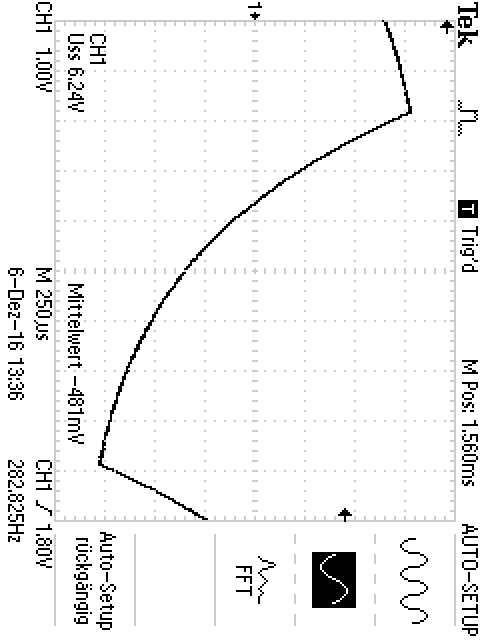
\includegraphics[angle=90]{bilder/F0000TEK.JPG}
	\caption{Aufgabenteil a: Bestimmung der Zeitkonstante $RC$}
	\label{fig:plotrc}
\end{figure}

\begin{figure}
  \centering
  \includegraphics{build/test.pdf}
  \caption{Lineare Regression zur Bestimmung der Zeitkonstanten $RC$}
  \label{fig:plota}
\end{figure}

\begin{figure}
  \centering
  \includegraphics{build/amplitude.pdf}
  \caption{Regression zur Bestimmung der Zeitkonstanten $RC$}
  \label{fig:plota}
\end{figure}

\subsection{d) Integration}

\begin{figure}
	\centering
	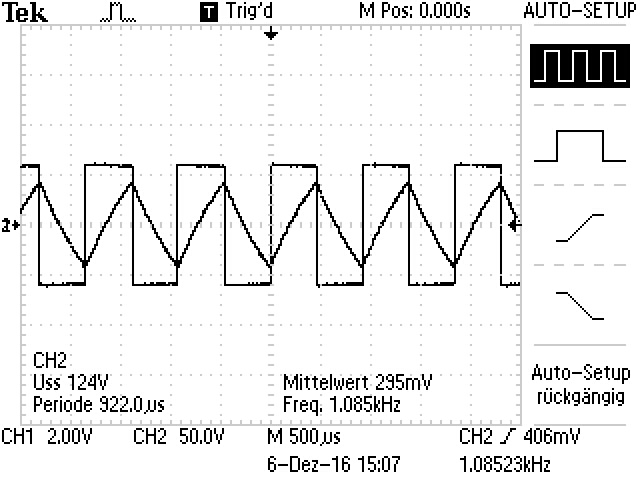
\includegraphics[angle=90]{bilder/ALL0001/F0001TEK.JPG}
	\caption{Aufgabenteil d: Rechteckspannung}
	\label{fig:rechteck}
\end{figure}

In Abbildung \ref{fig:rechteck} ist die Rechteckspannung sowie die über das RC-Glied integrierte Rechteckspannung dargestellt.
Die integrierte Rechteckspannung ist wie zu erwarten eine Dreiecksspannung.


\begin{figure}
	\centering
	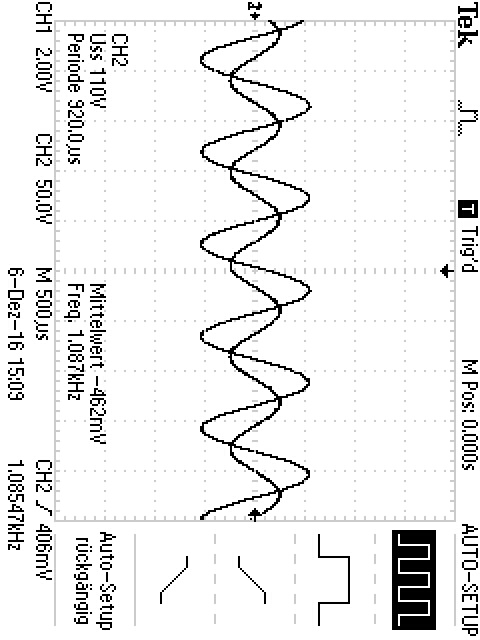
\includegraphics[angle=90]{bilder/ALL0002/F0002TEK.JPG}
	\caption{Aufgabenteil d: Sinusspannung}
	\label{fig:sinus}
\end{figure}

Der Spannungsverlauf der Sinusspannung ist in Abbildung \ref{fig:sinus} dargestellt. Wie zuvor ist die Kosinusspannung - integrierte Sinusspannung - außerdem in diesem Plot aufgezeichnet.


\begin{figure}
	\centering
	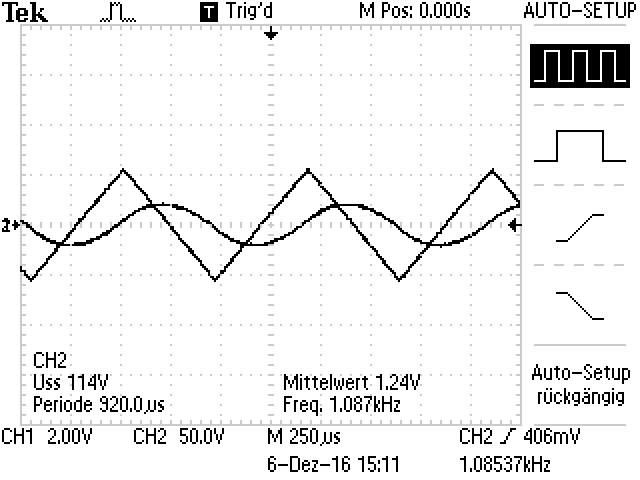
\includegraphics[angle=90]{bilder/ALL0003/F0003TEK.JPG}
	\caption{Aufgabenteil d: Dreiecksspannung}
	\label{fig:dreieck}
\end{figure}

In Abbildung \ref{fig:dreieck} ist Dreieck und Parabelspannung zu sehen
